\documentclass[12pt, twoside]{article}
\usepackage[francais]{babel}
\usepackage[T1]{fontenc}
\usepackage[latin1]{inputenc}
\usepackage[left=5mm, right=5mm, top=5mm, bottom=5mm]{geometry}
\usepackage{float}
\usepackage{graphicx}
\usepackage{array}
\usepackage{multirow}
\usepackage{amsmath,amssymb,mathrsfs}
\usepackage{textcomp}
\pagestyle{empty}
\usepackage{soul}

\begin{document} 

 
 
\begin{flushleft}
NOM PRENOM: \ldots \ldots \ldots \ldots \ldots \ldots \ldots \ldots \ldots
 

\end{flushleft} 
 
\bigskip

\begin{center}
{\fbox{$5^{e}2$ \qquad \qquad \textbf{\Large{Devoir surveill� 6 (sujet 1) }}
\qquad \qquad 21/05/2010}}
\end{center}

\textit{Remarque: la calculatrice est autoriss�e. Toutes les r�ponses doivent
�tre justifi�es (en notant votre calcul). Un r�sultat non expliqu� donnera 0
point.} Exercices 1 et 2 � faire sur la photocopie.

\enskip


\ul{Exercice 1}: (\textit{5 points})

\begin{enumerate}
  \item J, O, E, K sont quatre points tels que EJ=OE=EK. Compl�ter la phrase:
  
  
  ``Le point \ldots\ldots est le centre du cercle circonscrit au triangle
  \ldots \ldots''.
  \item Construire les cercles circonscrits aux triangles suivants:
 
  
   \bigskip
    
  \begin{tabular}{cc}
  \begin{minipage}{9cm}
  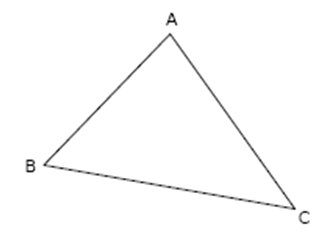
\includegraphics[width=5cm]{images/ex11.jpg}
  \end{minipage}
&
\begin{minipage}{9cm}
   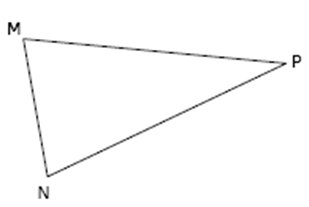
\includegraphics[width=5cm]{images/ex12.jpg}
  \end{minipage}
  \end{tabular}
   
  \end{enumerate}

\bigskip


\ul{Exercice 2}: (\textit{2 points})

\begin{enumerate}
  \item Donner la d�finition de la hauteur d'un triangle: \ldots \ldots \ldots
  \ldots \ldots \ldots  \ldots \ldots \ldots \ldots
  \ldots \ldots \ldots  \ldots  \ldots \ldots \ldots
  \ldots \ldots 
   
  \ldots \ldots \ldots \ldots \ldots \ldots  \ldots \ldots \ldots \ldots
  \ldots \ldots \ldots  \ldots  \ldots \ldots \ldots \ldots \ldots  \ldots
  \ldots \ldots \ldots \ldots \ldots  \ldots \ldots \ldots \ldots \ldots \ldots
  \ldots \ldots \ldots 
  
     \item Donner la formule permettant de calculer l'aire d'un triangle:   \ldots \ldots \ldots  \ldots \ldots \ldots \ldots
  \ldots \ldots \ldots  \ldots  \ldots \ldots \ldots  
       
\end{enumerate}


\bigskip


\ul{Exercice 3}: (\textit{2 points})  Calculer l'aire des triangles suivants:

\enskip

\begin{tabular}{c|c}
\begin{minipage}{12cm}

GE=3,8cm;  EF=4,4cm; FU=4cm; GU=2cm; EU=3,7cm

\begin{center}
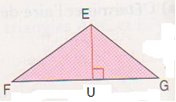
\includegraphics[width=3cm]{images/ex31.jpg}
\end{center}

\end{minipage}

&
\begin{minipage}{6cm}
\begin{center}
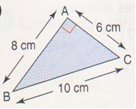
\includegraphics[width=3cm]{images/ex32.jpg}
\end{center}

\end{minipage}
\end{tabular}

\bigskip

\ul{Exercice 4}: (\textit{2 points})

\begin{tabular}{cc}
\begin{minipage}{14cm}

Le triangle DBC a pour aire 10,5$cm^2$ et DC=7cm. Calculer la longueur BH.

\end{minipage}

&
\begin{minipage}{4cm}
\begin{center}
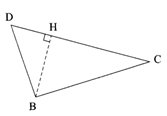
\includegraphics[width=35mm]{images/ex4.jpg}
\end{center}

\end{minipage}
\end{tabular}


\bigskip



\begin{tabular}{cc}
\begin{minipage}{8cm}
\ul{Exercice 5}: (\textit{3 points})

\begin{center}
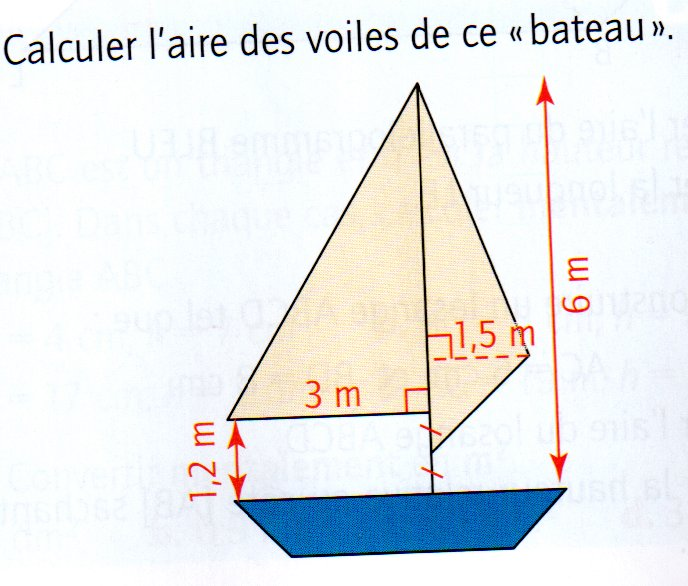
\includegraphics[width=6cm]{images/ex5.jpg}

\end{center}
\end{minipage}
&\begin{minipage}{10cm}
\ul{Exercice 6}: (\textit{6 points}) Effectuer les calculs en d�taillant les
�tapes:

\bigskip

\begin{center}
$A=\dfrac{1}{3}+\dfrac{4}{3}$ \qquad $B=\dfrac{4}{7}-\dfrac{1}{7}$ \qquad
$C=\dfrac{2}{5}+\dfrac{3}{10}$

\bigskip

$D=\dfrac{5}{6}-\dfrac{1}{12}$ \qquad
$E=4+\dfrac{3}{5}$ \qquad $F=\dfrac{7}{3}+\dfrac{5}{9}-2$


\end{center}
\end{minipage}
\end{tabular}



\pagebreak


 
\begin{flushleft}
NOM PRENOM: \ldots \ldots \ldots \ldots \ldots \ldots \ldots \ldots \ldots
 

\end{flushleft} 
 
\bigskip

\begin{center}
{\fbox{$5^{e}2$ \qquad \qquad \textbf{\Large{Devoir surveill� 6 (sujet 2) }}
\qquad \qquad 21/05/2010}}
\end{center}

\textit{Remarque: la calculatrice est autoriss�e. Toutes les r�ponses doivent
�tre justifi�es (en notant votre calcul). Un r�sultat non expliqu� donnera 0
point.} Exercices 1 et 2 � faire sur la photocopie.

\enskip


\ul{Exercice 1}: (\textit{5 points})

\begin{enumerate}
  \item K, L, M, T sont quatre points tels que KL=LM=LT. Compl�ter la phrase:
  
  
  ``Le point \ldots\ldots est le centre du cercle circonscrit au triangle
  \ldots \ldots''.
  \item Construire les cercles circonscrits aux triangles suivants:
 
  
   \bigskip
    
  \begin{tabular}{cc}
  \begin{minipage}{9cm}
  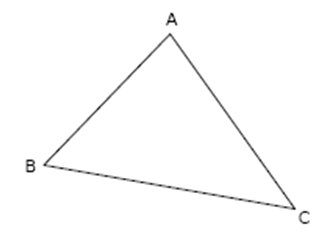
\includegraphics[width=5cm]{images/ex11.jpg}
  \end{minipage}
&
\begin{minipage}{9cm}
   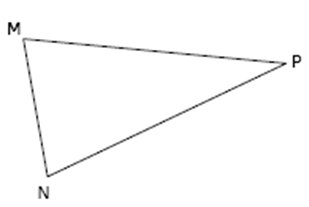
\includegraphics[width=5cm]{images/ex12.jpg}
  \end{minipage}
  \end{tabular}
   
  \end{enumerate}

\bigskip


\ul{Exercice 2}: (\textit{2 points})

\begin{enumerate}
  \item Donner la d�finition de la hauteur d'un triangle: \ldots \ldots \ldots
  \ldots \ldots \ldots  \ldots \ldots \ldots \ldots
  \ldots \ldots \ldots  \ldots  \ldots \ldots \ldots
  \ldots \ldots 
   
  \ldots \ldots \ldots \ldots \ldots \ldots  \ldots \ldots \ldots \ldots
  \ldots \ldots \ldots  \ldots  \ldots \ldots \ldots \ldots \ldots  \ldots
  \ldots \ldots \ldots \ldots \ldots  \ldots \ldots \ldots \ldots \ldots \ldots
  \ldots \ldots \ldots 
  
     \item Donner la formule permettant de calculer l'aire d'un triangle:   \ldots \ldots \ldots  \ldots \ldots \ldots \ldots
  \ldots \ldots \ldots  \ldots  \ldots \ldots \ldots  
       
\end{enumerate}


\bigskip


\ul{Exercice 3}: (\textit{2 points})  Calculer l'aire des triangles suivants:

\enskip

\begin{tabular}{c|c}
\begin{minipage}{12cm}

GE=3,6cm;  EF=5,4cm; FU=6cm; GU=3cm; EU=3,5cm

\begin{center}
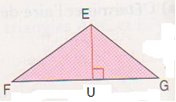
\includegraphics[width=3cm]{images/ex31.jpg}
\end{center}

\end{minipage}

&
\begin{minipage}{6cm}
\begin{center}
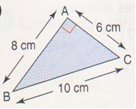
\includegraphics[width=3cm]{images/ex32.jpg}
\end{center}

\end{minipage}
\end{tabular}

\bigskip

\ul{Exercice 4}: (\textit{2 points})

\begin{tabular}{cc}
\begin{minipage}{14cm}

Le triangle DBC a pour aire 49,5$cm^2$ et DC=11cm. Calculer la longueur BH.

\end{minipage}

&
\begin{minipage}{4cm}
\begin{center}
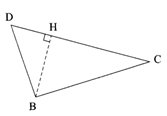
\includegraphics[width=35mm]{images/ex4.jpg}
\end{center}

\end{minipage}
\end{tabular}


\bigskip



\begin{tabular}{cc}
\begin{minipage}{8cm}
\ul{Exercice 5}: (\textit{3 points})

\begin{center}
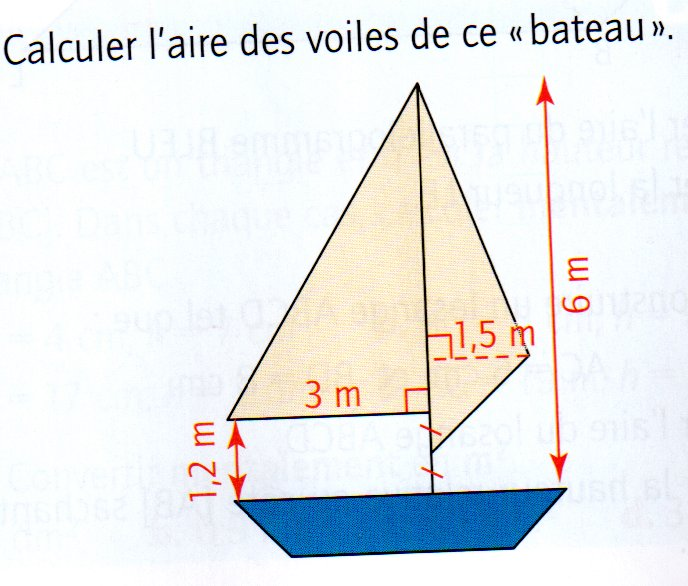
\includegraphics[width=6cm]{images/ex5.jpg}

\end{center}
\end{minipage}
&\begin{minipage}{10cm}
\ul{Exercice 6}: (\textit{6 points}) Effectuer les calculs en d�taillant les
�tapes:

\bigskip

\begin{center}
$A=\dfrac{1}{4}+\dfrac{3}{4}$ \qquad $B=\dfrac{4}{9}-\dfrac{1}{9}$ \qquad
$C=\dfrac{2}{6}+\dfrac{3}{12}$

\bigskip

$D=\dfrac{7}{10}-\dfrac{1}{5}$ \qquad
$E=3+\dfrac{5}{7}$ \qquad $F=\dfrac{7}{4}+\dfrac{5}{2}-3$


\end{center}
\end{minipage}
\end{tabular}

\end{document}
